\documentclass{beamer}

\usetheme{Frankfurt}
\usecolortheme{cormorant}
\title{Embedded Android Development}

\author{Fernando Ferreira Silva \\ \texttt{fernando@fer.dev.br}}

\begin{document}

\begin{frame}
  \titlepage
\end{frame}

\begin{frame}
  \frametitle{Revisão}
  \begin{itemize}
  \item Sistemas embarcados
  \item Sistemas operacionais
  \item Kernel Linux
  \item Android OS
  \item Compilação cruzada
  \end{itemize}  
\end{frame}

\begin{frame}
  \frametitle{O que é sistema embarcado}
  \begin{itemize}
  \item Contém uma ou mais unidades de processamento
  \item Customizado para um propósito específico
  \item Compõem um sistema maior
  \item Menos custo se comparado a um sistema generalista
  \end{itemize}
  Exemplo celular, com modem, bateria, giroscopio
  3 aproximações para resolver um problema

\end{frame}

\begin{frame}
  \frametitle{O que é sistema embarcado}
  \begin{itemize}
  \item Computador +  sensor
  \item SBC +  wifi +  sensor
  \item Placa Custom + sensor
  \end{itemize}
\end{frame}

\begin{frame}
  \frametitle{Tipos de sistemas embarcados}
  \begin{columns}
    \column{.5\textwidth}
    \begin{block}{Safety critical}
     \begin{itemize}
      \item Aplicação não complexa
      \item Exemplo: Freio ABS
      \item Vida humana em perigo
      \item Deterministic scheduling
      \item Bare metal, RTOS
      \end{itemize}
    \end{block}
    \column{.5\textwidth}
    \begin{block}{Non safety critical}
      \begin{itemize}
      \item Aplicação complexa
      \item Exemplo: Controlador Multimídia
      \item Problemas nas funcionalidades quando há defeito
      \item Não oferece risco a vida
      \item Linux, Android  
      \end{itemize}
    \end{block}
  \end{columns}
\end{frame}


\begin{frame}
  \frametitle{Desenvolvimento}
  \begin{itemize}
  \item Fabricante (vendor), NXP, ST, Rockchip, Intel
    \begin{itemize}
    \item Fabricam SoC (System On Chip)
    \item Disponibilizam plataformas de referencia
    \item Disponibilizam BSP (Board Support Package)
    \item Com objetivo de promover seus SoC's
    \end{itemize}
  \item Desenvolvedor
    \begin{itemize}
    \item Hardware customizado, baseado na plataforma de referencia
    \item Software customizado, baseado no BSP
    \end{itemize}
  \end{itemize}
\end{frame}

\begin{frame}
  \frametitle{Ambiente de desenvolvimento}
  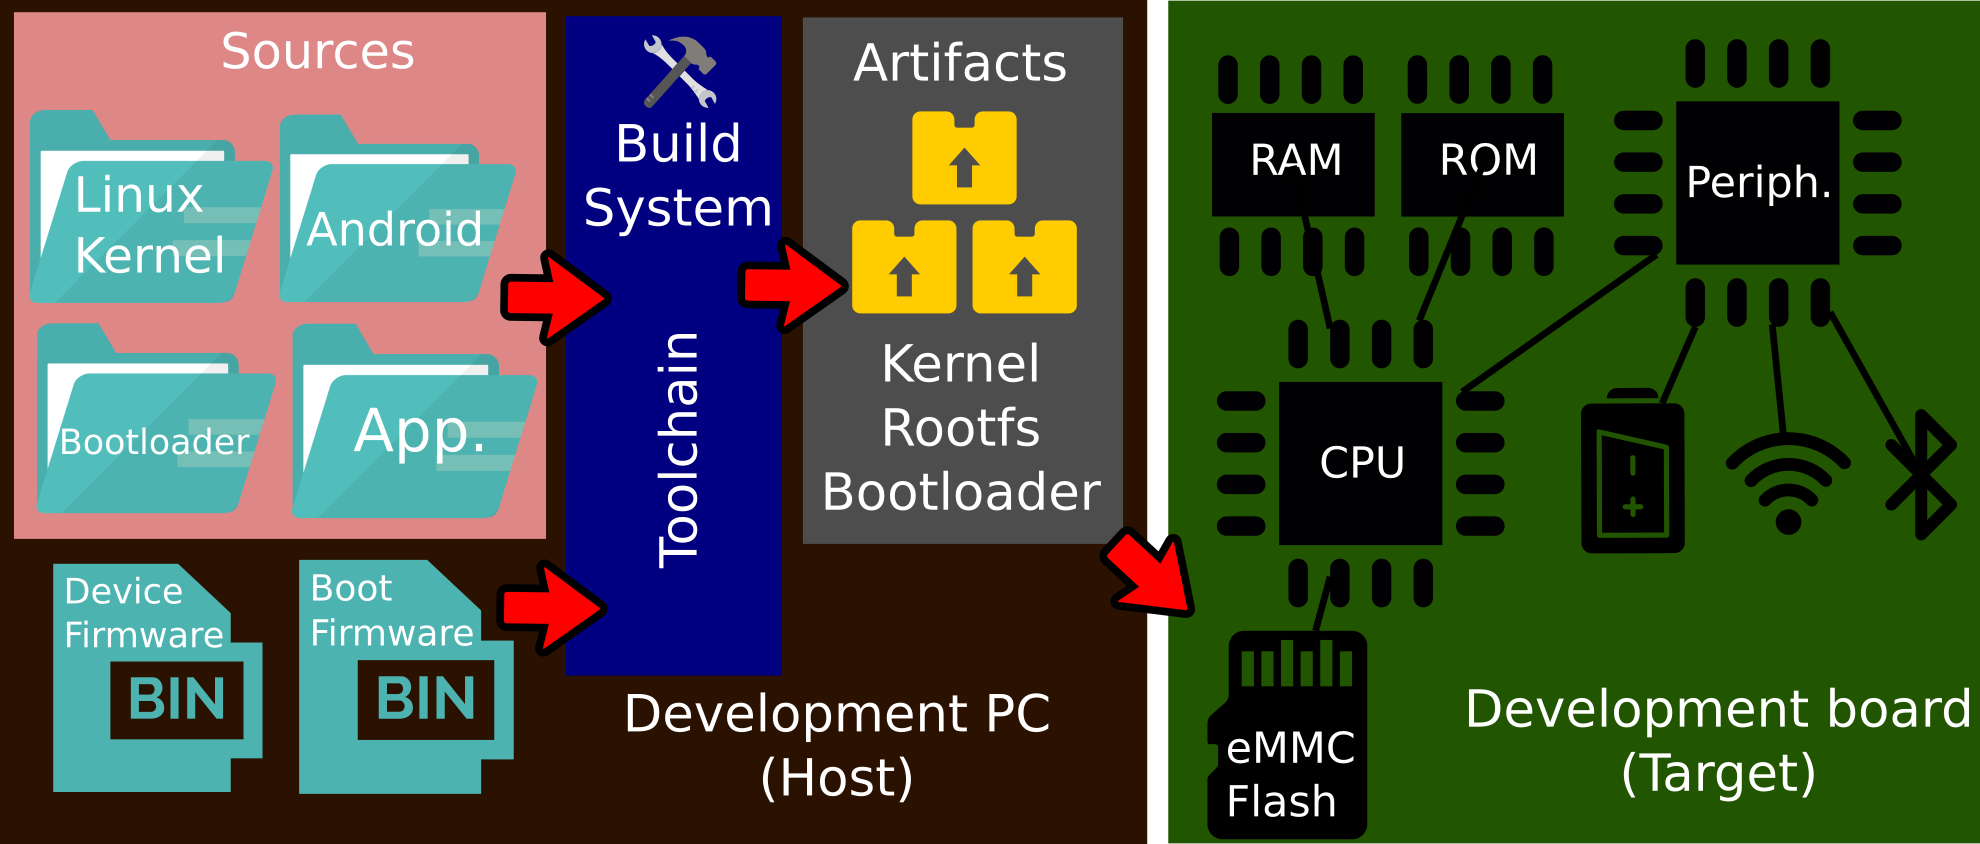
\includegraphics[width=\textwidth,height=\textheight,keepaspectratio]{./media/embedded_env.png}
\end{frame}

\begin{frame}
  \frametitle{Android vs Linux}
  \begin{itemize}
  \item Bionic C library
  \item OOM-killer
  \item Wakelocks
  \item Binder IPC
  \item HAL(Hardware Abstraction Layer)
  \item Mecanismo de log
  \end{itemize}
\end{frame}

\begin{frame}
  \frametitle{Linux Architecture}
  \begin{columns}
    \column{.5\textwidth}
    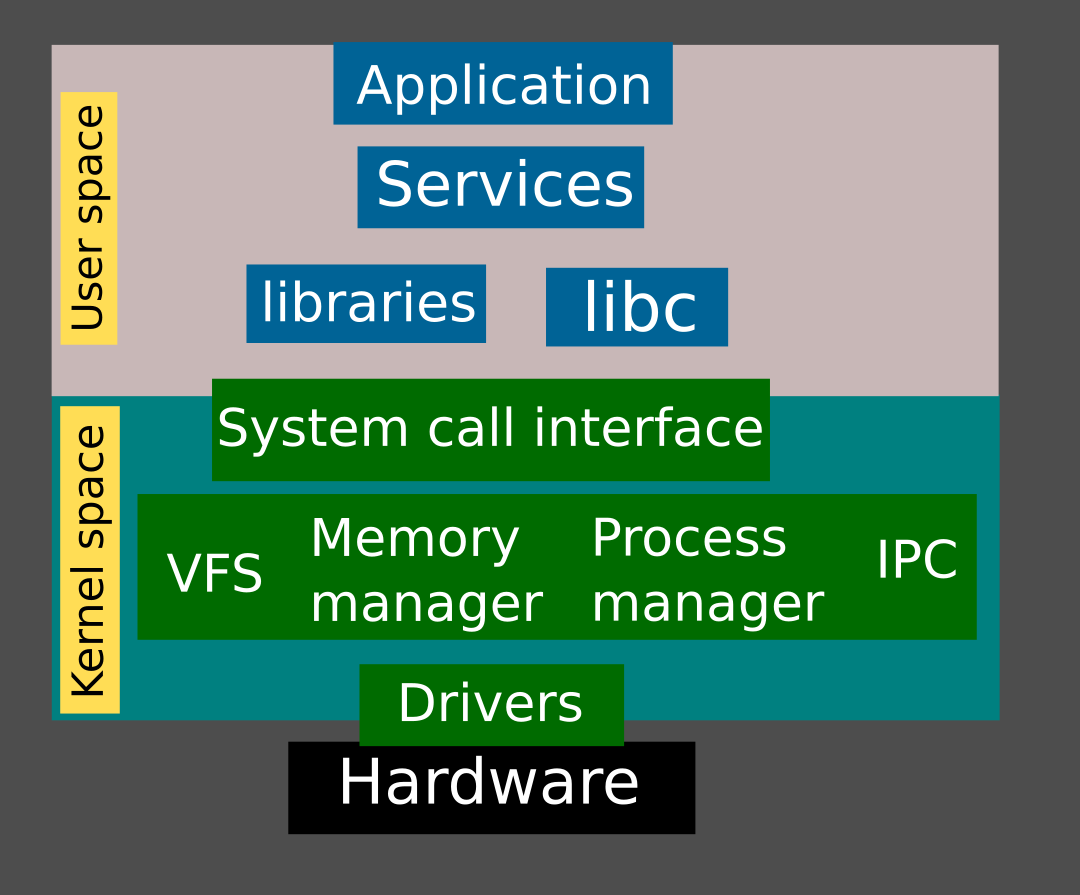
\includegraphics[width=\textwidth,height=\textheight,keepaspectratio]{./media/linux_arch.png}
    \column{.5\textwidth}
    \begin{block}{Ex: Network connection}
      \begin{itemize}
      \item{App: nmtui, ifconfig, plasma-nm}
      \item{Service: network-manager, wickedd}
      \item{Libraries: libudev, libnm}
      \item{Kernel: Eth or Wifi virtual device}
      \item{Driver: network card connection}
      \end{itemize}
    \end{block}
  \end{columns}
\end{frame}

\begin{frame}
  \frametitle{Android Architecture}
\end{frame}

\begin{frame}
  \frametitle{Boot process}
\end{frame}

\begin{frame}
  \frametitle{Hands on - virtual device}
  \begin{itemize}
  \item{tools}
  \item{Aosp sources}
  \item{Emulator}
  \end{itemize}
\end{frame}
    
  

\end{document}
